\documentclass[border=6pt]{standalone}
\usepackage{tikz}
\usetikzlibrary{arrows.meta,calc,decorations.pathreplacing}
\begin{document}
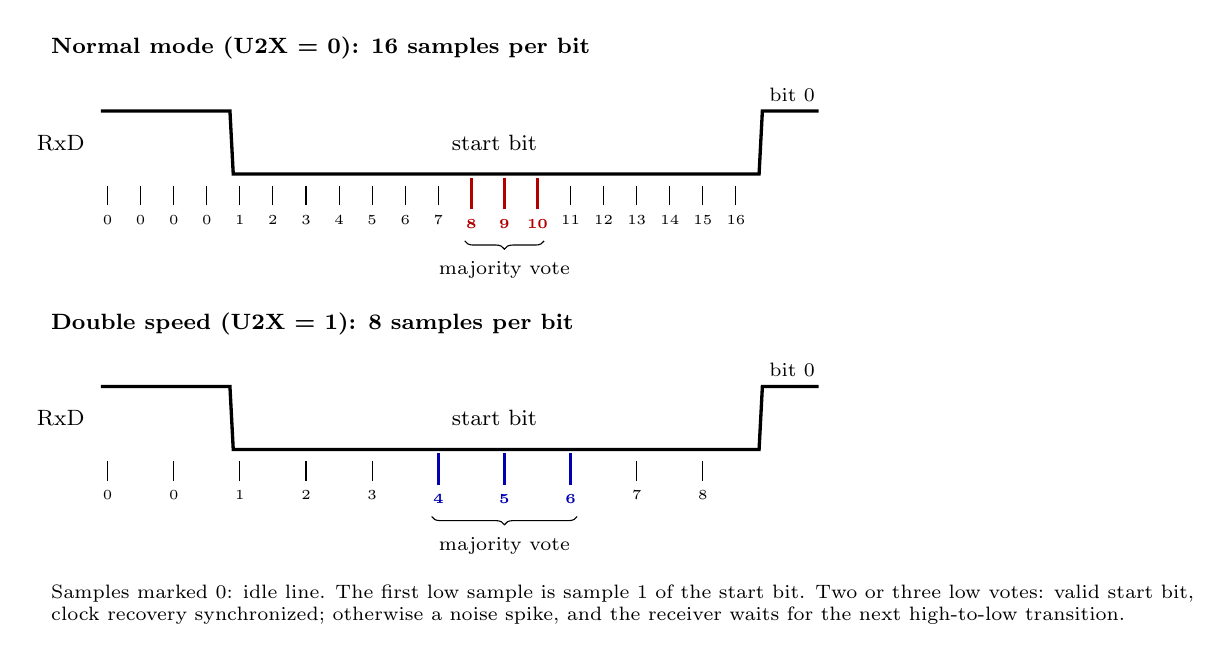
\begin{tikzpicture}[>=Stealth,font=\small,x=0.42cm,y=1cm]
% Normal mode: 16 samples per bit; sample k of the start bit at x = k-1
\def\h{0.8}
\node[font=\footnotesize\bfseries,anchor=west] at (-6,1.6) {Normal mode (U2X = 0): 16 samples per bit};
\node[anchor=east,font=\footnotesize] at (-4.4,0.4) {RxD};
\draw[very thick] (-4.2,\h) -- (-0.3,\h) -- (-0.2,0) -- (15.7,0) -- (15.8,\h) -- (17.5,\h);
\node[font=\footnotesize] at (7.7,0.4) {start bit};
\node[font=\scriptsize,anchor=south] at (16.7,\h) {bit 0};
\foreach \x in {-4,-3,-2,-1} { \draw (\x,-0.4) -- (\x,-0.15); \node[font=\tiny,below] at (\x,-0.4) {0}; }
\foreach \k in {1,...,16} {
  \pgfmathtruncatemacro{\v}{(\k>7)*(\k<11)}
  \ifnum\v=1 \draw[red!70!black,very thick] (\k-1,-0.45) -- (\k-1,-0.05); \node[font=\tiny\bfseries,red!70!black,below] at (\k-1,-0.45) {\k};
  \else \draw (\k-1,-0.4) -- (\k-1,-0.15); \node[font=\tiny,below] at (\k-1,-0.4) {\k}; \fi
}
\draw[decorate,decoration={brace,mirror,amplitude=3pt}] (6.8,-0.85) -- (9.2,-0.85) node[midway,below=4pt,font=\scriptsize]{majority vote};
% Double speed: 8 samples per bit, same time scale (each sample 2 units)
\begin{scope}[yshift=-3.5cm]
\node[font=\footnotesize\bfseries,anchor=west] at (-6,1.6) {Double speed (U2X = 1): 8 samples per bit};
\node[anchor=east,font=\footnotesize] at (-4.4,0.4) {RxD};
\draw[very thick] (-4.2,\h) -- (-0.3,\h) -- (-0.2,0) -- (15.7,0) -- (15.8,\h) -- (17.5,\h);
\node[font=\footnotesize] at (7.7,0.4) {start bit};
\node[font=\scriptsize,anchor=south] at (16.7,\h) {bit 0};
\foreach \x in {-4,-2} { \draw (\x,-0.4) -- (\x,-0.15); \node[font=\tiny,below] at (\x,-0.4) {0}; }
\foreach \k in {1,...,8} {
  \pgfmathtruncatemacro{\v}{(\k>3)*(\k<7)}
  \pgfmathsetmacro{\x}{2*\k-2}
  \ifnum\v=1 \draw[blue!70!black,very thick] (\x,-0.45) -- (\x,-0.05); \node[font=\tiny\bfseries,blue!70!black,below] at (\x,-0.45) {\k};
  \else \draw (\x,-0.4) -- (\x,-0.15); \node[font=\tiny,below] at (\x,-0.4) {\k}; \fi
}
\draw[decorate,decoration={brace,mirror,amplitude=3pt}] (5.8,-0.85) -- (10.2,-0.85) node[midway,below=4pt,font=\scriptsize]{majority vote};
\end{scope}
\node[font=\scriptsize,align=left,anchor=north west] at (-6,-5.1) {Samples marked 0: idle line. The first low sample is sample 1 of the start bit. Two or three low votes: valid start bit,\\clock recovery synchronized; otherwise a noise spike, and the receiver waits for the next high-to-low transition.};
\end{tikzpicture}
\end{document}
